\documentclass{standalone}
\usepackage{pgfplots}
\pgfplotsset{compat=newest}

\begin{document}
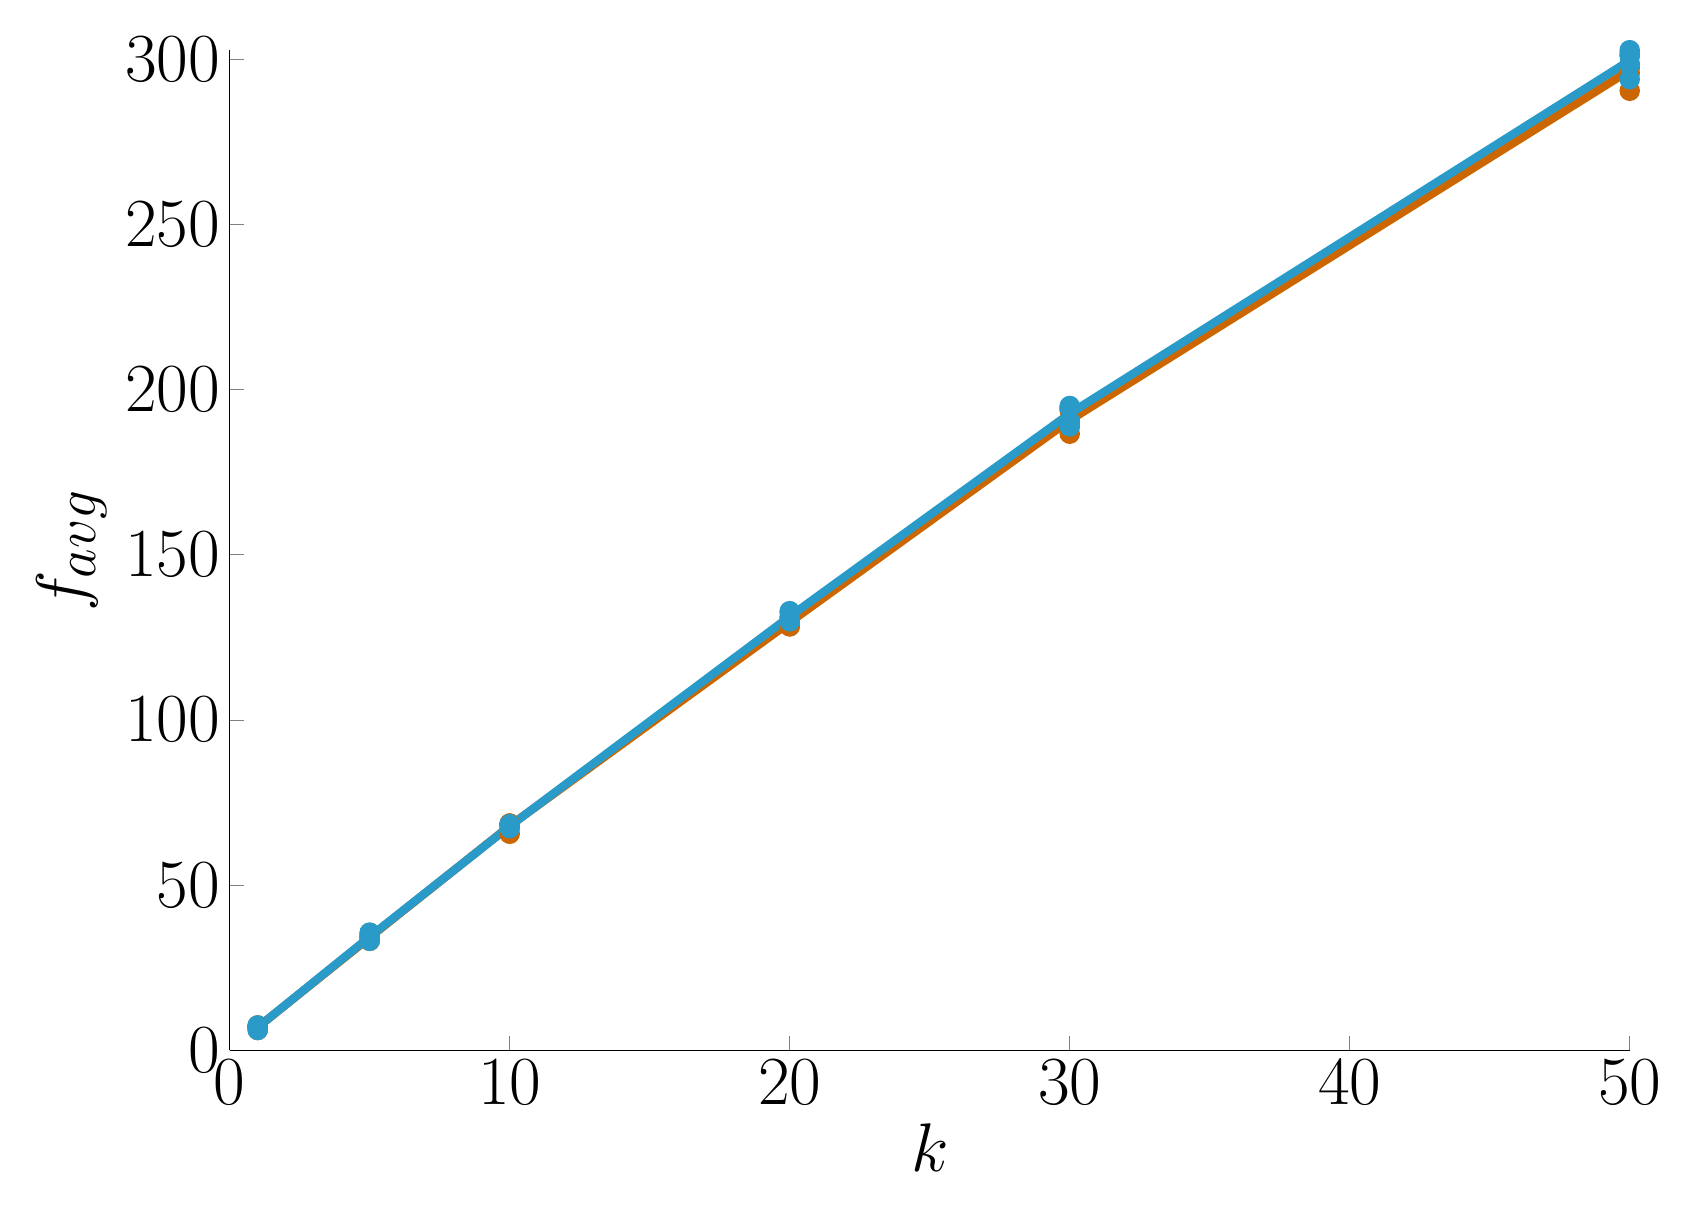
\begin{tikzpicture}

\begin{axis}[%
tick label style={font=\Huge},
label style={font=\Huge},
legend style={font=\Huge},
view={0}{90},
max space between ticks=50pt,
width=7in,
height=5in,
scale only axis,
xmin=0, xmax=50,
xtick={0, 10, 20, 30, 40, 50},
xlabel={$k$},
ymin=0, ymax=302.7,
%ytick={0, 200, 400, 600, 800, 1000},
ylabel={$f_{avg}$},
major tick length=5pt,
axis lines*=left,
legend cell align=left,
clip=false]

\addplot [
only marks,
mark=*,
mark size=3.5pt,
color=orange!80!black,
%solid,
%line width=2pt,
]
coordinates{
(1,6.1)(1,6.7)(1,7.0)(1,7.3)(1,7.5)(5,33.1)(5,33.5)(5,34.3)(5,34.3)(5,35.4)(10,65.5)(10,68.3)(10,68.5)(10,68.6)(10,68.6)(20,128.3)(20,128.3)(20,129.9)(20,130.0)(20,131.0)(30,186.6)(30,188.9)(30,190.1)(30,193.6)(30,194.1)(50,290.4)(50,295.7)(50,297.3)(50,298.5)(50,301.1)
};

\addplot [
only marks,
mark=*,
mark size=3.5pt,
color=cyan!80!black,
%solid,
%line width=2pt,
]
coordinates{
(1,6.1)(1,6.7)(1,7.0)(1,7.3)(1,7.5)(5,33.1)(5,33.5)(5,34.5)(5,34.9)(5,35.6)(10,67.2)(10,67.6)(10,67.8)(10,68.0)(10,68.4)(20,129.8)(20,129.9)(20,131.2)(20,132.5)(20,132.9)(30,188.8)(30,190.5)(30,194.4)(30,194.7)(30,195.0)(50,293.9)(50,298.3)(50,301.0)(50,301.9)(50,302.7)
};

\addplot [
color=orange!80!black,
solid,
line width=3pt
]
coordinates{
(1,6.92)(5,34.12)(10,67.9)(20,129.5)(30,190.66)(50,296.6)
};

\addplot [
color=cyan!80!black,
solid,
line width=3pt
]
coordinates{
(1,6.92)(5,34.32)(10,67.8)(20,131.26)(30,192.68)(50,299.56)
};


\end{axis}
\end{tikzpicture}
\end{document}
